\section{实验}

\subsection{数据集}
LM-O数据集\cite{lmo}引入了具有不同遮挡程度的挑战性测试场景,包含各种颜色、形状和大小的家用物品。这种复杂性因不同程度的遮挡而加剧。该数据集包含1214张图像,仅用于测试,通过标注8个物体在部分遮挡下的位姿,显著提高了难度。这一增加极大地增加了位姿估计任务的复杂性。由于LM-O数据集中的训练图像数量有限,根据物体的CAD模型,BOP挑战赛创建了大量合成图像用于训练。位姿估计方法的性能受到仿真图像和真实图像之间域差距的极大影响,突显了域随机化和适应策略的重要性。借助公开可用的基于物理渲染(PBR)训练图像\cite{hodan2024bop},我们利用这些资源来弥合域差距,提高了训练方法的有效性。

\subsection{指标}
我们选择ADD(-S)误差指标作为6DoF姿态估计任务中最广泛使用的度量标准。该指标计算使用预测姿态和使用真实姿态投影到相机域中的模型点之间的平均距离。对于对称物体,该指标识别使用真实姿态投影的最近模型点,而不是匹配相同的模型点。在本文的所有实验中,如果ADD(-S)误差小于物体直径的$10\%$,则预测的姿态被认为是准确的,这是最常接受的阈值。

此外,我们使用BOP挑战赛定义的BOP评分指标\cite{hodan2024bop}。该评估采用三个指标:可见表面差异(VSD)、最大对称感知表面距离(MSSD)和最大对称感知投影距离(MSPD)。这三个指标的平均值,称为AR,作为整体性能指标。

\subsection{与现有技术的比较}

我们将我们的结果与其他仅使用仿真数据进行训练的方法进行比较,重点关注LM-O数据集\cite{lmo}。我们报告ADD(-S)的召回率百分比,并与LM-O数据集上的最新技术进行基准测试,如\autoref{tab:lmo_adds}所述。术语“RGB”表示输入中未使用深度信息,而“RGB-D”表示包含深度信息。我们使用BOP挑战赛2023\cite{hodan2024bop}提供的默认检测。我们的结果在平均性能方面接近最新方法HiPose,并在ape和glue物体上表现出优越的结果。

\begin{table}
    \centering
\caption{与最新技术在 LM-O上的比较}
\resizebox{\textwidth}{!}{%
    \begin{tabular}{c|c|c|c|c|c|c|c|c}
    \toprule 
    \multirow{2}{*}{Method} & \multicolumn{2}{c|}{RGB Input} & \multicolumn{5}{c}{RGB-D Input} \\ 
         \cline{2-9}
      & GDR-Net~\cite{wang2021gdr} 
& ZebraPose~\cite{su2022zebrapose}&  PR-GCN~\cite{Zhou2021PRGCNAD} 
& FFB6D~\cite{he2021ffb6d} 
& RCVPose~\cite{wu2022vote} 
& DFTr~\cite{zhou2023deep} & HiPose~\cite{2024hipose} & Ours\\
    \midrule
     ape & 46.8 
& 57.9& 40.2 
& 47.2 
&  60.3 
& 64.1 &  78.0 & \textbf{78.2}\\
     can & 90.8 
& 95.0& 76.2 
& 85.2 
&  92.5 
& 96.1 &  \textbf{98.9} & \textbf{98.9}  \\
     cat & 40.5 
& 60.6& 57.0 
& 45.7 
&  50.2 
& 52.2 &  \textbf{87.5} & 85.7\\
     driller & 82.6 
& 94.8& 83.2 
& 81.4 
&  78.2 
& 95.8 &  \textbf{97.8} & 97.7\\
     duck & 46.9 
& 64.5& 30.0 
& 53.9 
&  52.1 
& 72.3 &  \textbf{85.3} & 85.0\\
     eggbox* & 54.2 
& 70.9& 68.2 
& 70.2 
&  \textbf{81.2} 
& 75.3 &  80.3 & 80.7\\
     glue* & 75.8 
& 88.7& 67.0 
& 60.1 
&  72.1 
& 79.3 & 94.1 & \textbf{94.2}\\
     holepuncher & 60.1 
& 83.0& 97.2 
& 85.9 
& 75.2 
& 86.8 &  \textbf{95.2} & \textbf{95.2} \\
     \midrule
     mean & 62.2 & 76.9&  65.0 &  66.2 &  70.2 & 77.7 & \textbf{89.6} & 89.4\\
    \bottomrule
  \end{tabular}
  }
  \label{tab:lmo_adds}
\end{table}



我们还报告了BOP评分的结果,如\autoref{tab:lmo_bop}所示。我们的方法在准确性上与SurfEmb\cite{haugaard2022surfemb}相当,但我们的执行速度远远超过SurfEmb。向上箭头(↑)表示较高的指标值表示更好的性能,而向下箭头(↓)表示相反。术语“PBR”表示模型仅在合成图像上训练。

\begin{table}[htbp]
        \centering
        \caption{
                LM-O 数据集上的 BOP 结果
        }
        \resizebox{\textwidth}{!}{%
        \begin{tabular}{l c c c c c c c c}
        \toprule
        6D 物体位姿估计方法 & 输入类型 & 训练类型 &$AR\uparrow$&$AR_{VSD}\uparrow$&$AR_{MSSD}\uparrow$&$AR_{MSPD}\uparrow$&时间 (秒)$\downarrow$\\
        \midrule
        CDPNv2\cite{li2019cdpn} & RGB-D & pbr & 	63.0	&46.9&	68.9&	73.1&	0.506 \\
        FFB6D\cite{he2021ffb6d} & RGB-D & pbr & 68.7 & 55.0 & 71.8	& 79.2	& 0.189 \\
        DPODv2\cite{Shugurov2021DPODv2} & RGB-D & pbr & 70.0&	56.5&	74.8&	78.8&	0.334 \\
        CosyPose\cite{labbe2020cosypose} & RGB-D & pbr & 71.4 &	56.7 &	74.8 &	82.6 &	8.289 \\
        CIR\cite{lipson2022coupled} & RGB-D & pbr & 	73.4	&60.1&	77.8&	82.4	&-1.000 \\
        SurfEmb\cite{haugaard2022surfemb} & RGB-D & pbr &	76.0&	61.5&	80.9&	85.6&	11.943 \\
        \midrule
        BCFN (Ours) & RGB-D& pbr & 75.7 & 60.4 & 81.3 & 85.5 & 0.197\\
        \bottomrule
        \end{tabular}
        }
\label{tab:lmo_bop}
\end{table}
\subsection{消融研究}
\begin{table}[htbp]
  \centering
  \caption{关于设计设置的消融研究}
  \begin{tabular}{lccc}
  \toprule 
  & $128\times128$ & $256\times256$ & + 跳连接 \\
  \midrule
  ape & 76.76 & 77.02 & \textbf{77.28} \\
  can & 98.01 & \textbf{98.43} & 98.26 \\
  cat & 82.50 & 82.24 & \textbf{83.46} \\
  driller & 97.28 & \textbf{97.61} & 97.45 \\
  duck & 82.26 & 83.53 & \textbf{83.71} \\
  eggbox & 76.78 & 78.45 & \textbf{79.24} \\
  glue & 93.23 & \textbf{93.82} & \textbf{93.82} \\
  holepuncher & \textbf{95.12} & \textbf{95.12} & \textbf{95.12} \\
  \midrule
  均值 & 87.74 & 88.28 & \textbf{88.54} \\
  \bottomrule
  \end{tabular}
  \label{tab:main_ablation}
\end{table}
我们研究了各种超参数对ADD(-S)结果的影响,如\autoref{tab:main_ablation}所述。

\textbf{输出分辨率的影响 }输入图像被裁剪成边长为256像素的正方形。通过修改上采样层的数量,我们评估了CNN头输出配置在$128 \times 128$和$256 \times 256$分辨率下的效果。较大的CNN头尺寸导致了$0.5\%$的改进。

\textbf{跳跃连接 } 基线网络在CNN分支中缺少跳跃连接。我们尝试在具有相同维度的编码器和解码器层之间实现跳跃连接,具体方法是将编码器的输出与某些解码器层连接。引入跳跃连接后,性能提升了$0.26\%$。

\begin{table}
    \centering
    \caption{Influence of Consistent Loss}
    \begin{tabular}{lc}
    \toprule 
    Settings & ADD(-S) \\
    \midrule
    batch size = 16 w/o consistent loss & 87.95 \\
    batch size = 16 with consistent loss & 88.09 \\
    \midrule
    batch size = 32 w/o consistent loss & 88.05 \\
    batch size = 32 with consistent loss & 88.17 \\
    \bottomrule
  \end{tabular}
  \label{tab:consistent_loss}
\end{table}

\textbf{一致性损失 } 我们的标准训练批次大小设置为32。如~\cref{tab:consistent_loss}所示,我们报告了在批次大小为16和24的情况下,应用和不应用一致性损失的结果。结果证实了引入一致性损失的一致有效性。

\textbf{骨干网络 } 我们将ResNet-34骨干网络与ConvNeXt骨干网络进行了比较,观察到$0.73\%$的改进。

\subsection{可视化}

\begin{figure}[htbp]
\centerline{\includegraphics[width=\textwidth]{figure/bcfn/visualization.jpg}}
    \caption{可视化结果}
    \label{fig:visualization}
\end{figure}

我们在\autoref{fig:visualization}中展示了我们的定性结果。第一和第三行显示了输入图像,而第二和第四行展示了根据估计姿态渲染在调暗图像上的目标模型。

在\autoref{fig:vis_middle}中,我们展示了一个网络工作示例。最左边的图像是输入图像。在中间的点云图像中,红色和蓝色点云共同构成输入点云。我们的BCFN网络区分点云上的每个点是否属于物体。在这个示例中,红点表示物体上的点,而蓝点表示背景。对于每个红点,网络输出一个二进制编码,该编码可以进一步对应于物体坐标系下的坐标,表示为绿色点云。利用黑线指示的对应关系,我们使用Kabsch算法确定目标物体的姿态,如右图所示。

\begin{figure}[htbp]
\centerline{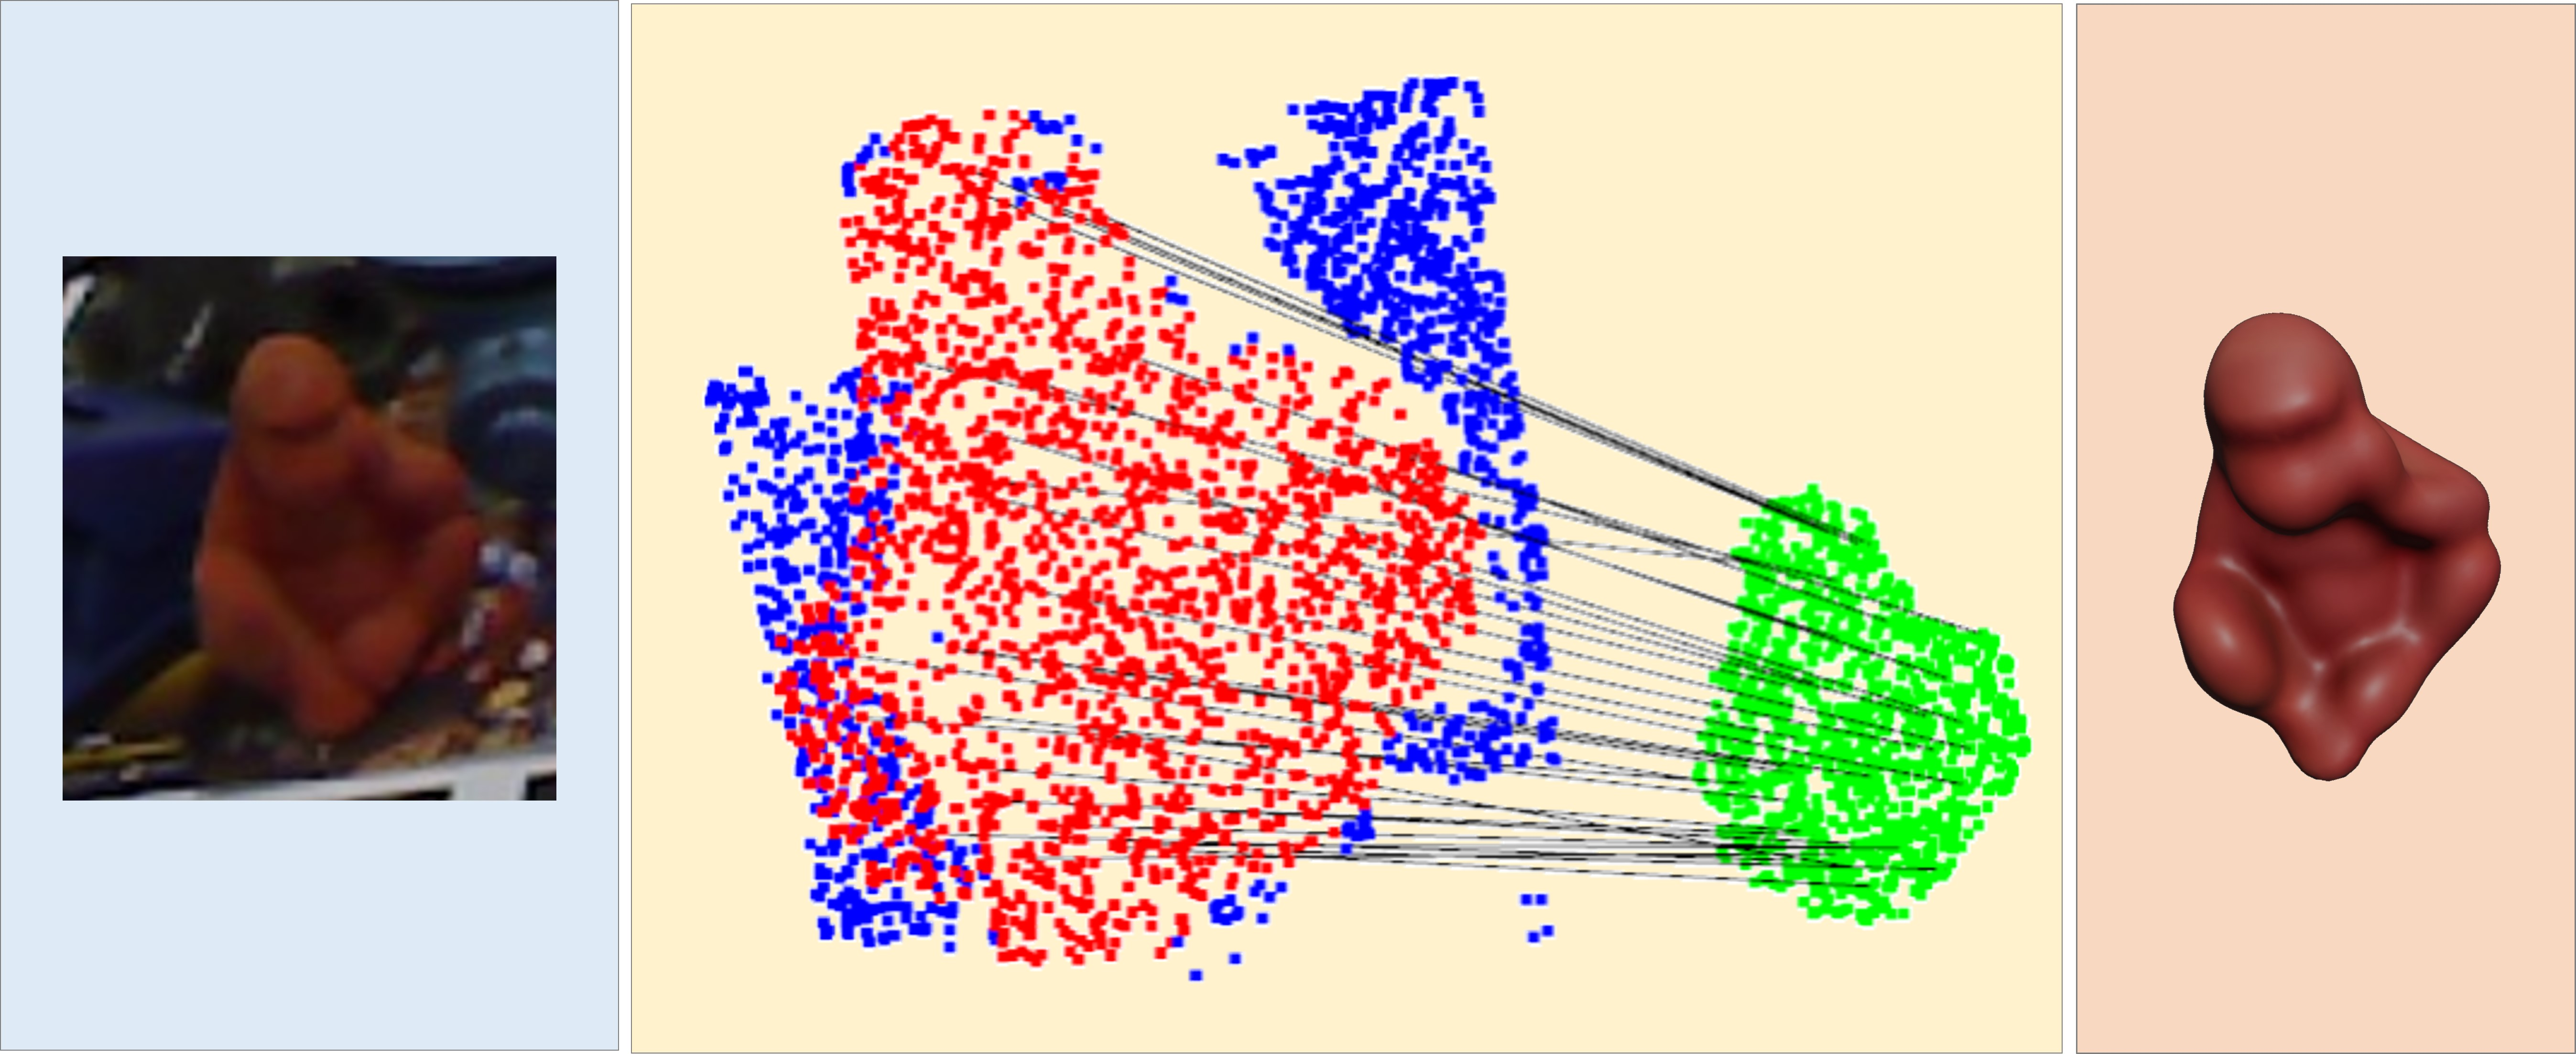
\includegraphics[width=0.80\textwidth]{figure/bcfn/vis_middle.jpg}}
    \caption{网络工作示例}
    \label{fig:vis_middle}
\end{figure}
